\section{Macchine di Turing}
\subsection{La Tesi di Church-Turing}
Finora abbiamo visto DFA con una quantità finita di memoria. I PDA che hanno memoria illimitata ma ad accesso limitato (abbiamo solo operazioni *push* e *pop*).
Questo comporta dei limiti alla loro capacità di computazione. 

\subsection{Macchina di Turing}
È un modello proposto da Alan Turing nel 1936 per risolvere problemi matematici.
\begin{itemize}
	\item Ha memoria illimitata, utilizza un nastro infinitoj/
	\item Non ci sono restrizioni di accesso alla memoria
\end{itemize}
Una macchina di Turing è un modello molto più preciso di un computer. 

\g{Tuttavia...}
\begin{itemize}
	\item Ci sono problemi che una Macchina di Turing **non può risolvere**
	\item questi problemi *vanno oltre le capacità di un computer*
\end{itemize}
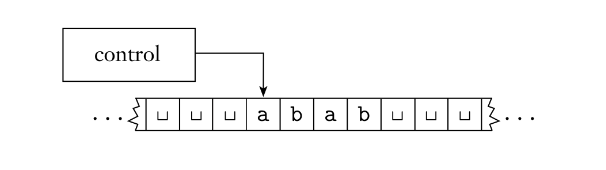
\includegraphics[scale=0.5]{img/schema_TM.png}

la macchina di Turing è composte da 
\begin{itemize}
	\item un nastro infinito come **memoria illimitata**
	\item una testina che **legge e scrive** simboli sul nastro
	\item all'inizio il nastro contiene l'input
	\item per memorizzare informazione si **scrive sul nastro** 
	\item la testina si può muovere **ovunque sul nastro**
	\item stati speciali per \g{accetta} e \g{rifiuta} 
\end{itemize}

\subsection{Primo esempio di TM}
Costruiamo una macchina di Turing per il linguaggio 
$$ B = \Big\{ w\# w \mid w\in \{0,1\}^* \Big\}$$
\begin{itemize}
	\item $M_1$deve accettare se l'input sta in $B$, e rifiutare altrimenti
	\item $M_1$= ''su input $w$:
\end{itemize}
\begin{enumerate}
	\item Si muove a zig-zag lungo il nastro, raggiungendo posizioni corrispondenti ai due lati di $\#$ per controllare se contengono lo stesso simbolo. In caso negativo, o se non trovi $\#$, \g{rifiuta}.
		Barra gli elementi già controllati 
	\item Se tutti i simboli a sinistra di $\#$ sono stati controllati, verifica i simboli a destra di $\#$. Se c'è qualche simbolo ancora da controllare \g{rifiuta}, altrimenti \g{accetta} 
\end{enumerate}
Questa descrizione della macchina di Turing $M_1$ ne illustra il funzionamento ma non ne mostra tutti i dettagli. 

\subsection{Automi finiti vs Macchine di Turing}
\begin{enumerate}
	\item Una TM può sia scrivere che leggere sul nastro
	\item  Una TM può muoversi si a a destra che a sinistra
	\item  Il nastro è infinito
	\item  Gli stati di rifiuto e accettazione hanno effetto immediato
\end{enumerate}

\subsection{Definizione formale}
Una macchina di Turing è una tupla $M = \{Q, \Sigma, \Gamma,\delta, q_0, q_{accept},q_{reject}\}$ 
	\begin{itemize}
	\item $Q$ è l'insieme finito di **stati**
	\item $\Sigma$ è l'**alfabeto di input** che non contiene il simbolo **blank**
	\item $\Gamma$ è l'**alfabeto del nastro** che contiene $\textvisiblespace$ e $\Sigma$ 
	\item $\delta : Q\times \Gamma\rightarrow Q\times\Gamma\times\{L,R\}$ è la **funzione di transizione** 
	\item $q_0\in Q$ è lo  **stato iniziale** 
	\item $q_{accept}\in Q$ è lo **stato di accettazione**
	\item $q_{reject}\in Q$ è lo **stato di rifiuto** (necessariamente diverso da $q_{accept}$ )
\end{itemize}
Nella macchina di Turing la funzione di transizione è la parte fondamentale. 

\subsection{Configurazioni}
Lo stato corrente, la posizione della testina e il contenuto del nastro formano a **configurazione** di una TM.
Dalla configurazione possiamo sapere la \g{prossima mossa}
Le configurazioni sono rappresentate da una tripla $uqv$:
\begin{itemize}
	\item $q$ è lo **stato corrente**
	\item $u$ è il contenuto del **nastro prima della testina** 
	\item $v$ è il contenuto del **nastro dalla testina in poi** 
	\item la testina si trova **sul primo simbolo di** $v$ 
\end{itemize}

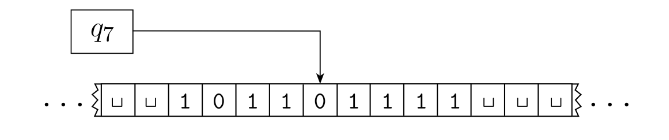
\includegraphics[scale=0.5]{img/tm_conf.png}
(la configurazione in figura è $1011q_701111$)

\subsection{Computazione}
La configurazione $C_1$ \b{produce} $C_1$ se la TM può passare da $C_1$ a $C_2$ in un passo
Se $a,b,c\in\Gamma$, $u,v\in\Gamma^*$ e $q_i, q_j$ sono stati, allora
	$uaq_ibv$ produce $uq_jacv$ se $\delta(q_i, b)= (q_i, c, L)$ 
	$uaq_ibv$ produce $uacq_jv$ se $\delta(q_i, b)= (q_i, c, R)$ 
\begin{itemize}
	\item la \g{configurazione iniziale} con input $w$ è $q_0w$ 
	\item in una \g{configurazione di accettazione} lo stato è $q_{accept}$ 
	\item in una \g{configurazione di rifiuto} lo stato è $q_{reject}$
\end{itemize}
\subsection{Linguaggi Turing-riconoscibili}
Una TM $M$ \g{accetta} l'input $w$ se esiste una **sequenza di configurazioni** $C_1, C_2,\dots, C_k$ tale che: 
\begin{itemize}
	\item $C_1$ è la configurazione iniziale con input $w$ 
	\item Ogni $C_i$ produce $C_{i+1}$ 
	\item $C_k$ è una configurazione di accettazione
\end{itemize}
Il \g{Linguaggio riconosciuto da} \textit{M} è l'insieme delle stringhe accettate da $M$ 

\begin{theorem}
	Un linguaggio è <i>Turing-riconoscibile</i> (o anche <i>ricorsivamente enumerabile</i>) se esiste una macchina di Turing che lo riconosce
\end{theorem}
</center>

\subsection{Linguaggi Turing-decidibili}
Se forniamo un input ad una TM, ci sono \g{tre risultati possibili}:
\begin{itemize}
	\item la macchina \g{accetta}
	\item la macchina \g{rifiuta} 
	\item la macchina va in \g{loop} e non si ferma mai
\end{itemize}
La TM può non accettare sia rifiutando che andando in loop.
Un TM che termina sempre la computazione è un \g{decisore} 
Un decisore \g{decide} un linguaggio se lo riconosce 

\begin{theorem}
	Un linguaggio è <i>Turing-decidibile</i> (o anche <i>ricorsivo</i>) se esiste una macchina di Turing che lo decide
\end{theorem}

\subsection{Esempi}
\subsubsection{Esempio 1}
TM che \g{decide} il linguaggio di tutte le stringhe di $0$ la cui lunghezza è una potenza di 2:
$$A = \{0^{2^n}\mid n\geq 0\}$$
$M_1=$ "su input $w$: 
\begin{enumerate}
	\item Scorri il nastro da sinistra a destra, cancellando ogni secondo $0$ 
	\item Se il nastro conteneva un solo $0$, \g{accetta}
	\item Se il nastro conteneva un numero dispari di $0$, \textit{rifiuta}
	\item  Ritorna all'inizio del nastro
	\item  Vai al passo 1"
\end{enumerate}

\subsubsection{Esempio 2}
% link primo esempio di TM
vedi Primo esempio di TM

\subsubsection{Esempio 3}
TM che esegue operazioni aritmetiche.  Decide il linguaggio
$C=\{a^ib^jc^k\mid k = i\cdot j$ e $i,j,k\geq 1\}$ 

$M_3=$ "su input $w$:
\begin{enumerate}
	\item Scorri il nastro da sinistra a destra e controlla se l'input sta in $a^+b^+c^+$. \g{rifiuta} se non lo è
	\item Ritorna all'inizio del nastro
	\item Barra una $a$ e scorri a destra fino a trovare una $b$. Fai la spola tra $b$ e $c$, barrando le $b$ e le $c$ fino alla fine delle $b$. Se tutte le $c$ sono barrate e rimangono ancora $b$, \textit{rifiuta}.
	\item Ripristina le $b$ barrate e ripeti \item finché ci sono $a$ da barrare.
	\item Quando tutte le $a$ sono barate, controlla se tutte le $c$ sono barrate: se sì, \g{accetta}; altrimenti \textit{rifiuta}."
\end{enumerate}

\subsubsection{Esempio 4}
TM che risolve il problem degli **elementi distinti**. Prende in input una sequenza di stringhe separate da $\#$ e accetta se tutte le stringhe sono diverse. 
Decide il linguaggio:
$D=\{\#x_1\#x_2\#\dots\#x_l\mid x_j\in \{0,1\}^*$ e $x_i\neq x_j$ per ogni $i\neq j\}$ 

$M_4=$ "su input $w$ 
\begin{enumerate}
	\item Mette un segno sul simbolo del nastro più a sinistra. Se è un blank, \g{accetta}. Se è un $\#$, continua con \item Altrimenti, \textit{rifiuta}.
	\item Scorre a destra fino al successivo $\#$ e vi mette sopra un secondo segno. Se nessun $\#$ viene trovato, allora era presente solo $x_1:$ \g{accetta}.
	\item Procede a zig-zag confrontando le due stringhe a destra dei $\#$ segnati. Se sono uguali, \g{rifiuta}
	\item Sposta il segno più a destra sul successivo $\#$ alla sua destra.Se non trova nessun $\#$, sposta il segno più a sinistra sul successivo $\#$ alla sua destra, e sposta il segno più a destra sul successivo $\#$. Se on c'è un $\#$ dopo il segno più a destra, allora tutte le stringhe sono state confrontate: \g{accetta}
	\item Vai alla fase 3.
\end{enumerate}

\subsection{Conclusioni}
\begin{itemize}
	\item I linguaggi $A, B, C$ e $D$ sono \textit{decidibili}
	\item Tutti i linguaggi Turing-decidibili sono anche Turing-riconoscibili
	\item I linguaggi $A,B,C$ e $D$ sono anche \textit{Turing-riconoscibili}
	\item Vedremo che ci sono linguaggi \textit{Turing-riconoscibili ma non decidibili}
\end{itemize}

